\documentclass[12pt,english]{beamer}
\usepackage[utf8]{inputenc}
\usepackage[T1]{fontenc}
\usepackage{booktabs}
\usepackage{babel}
\usepackage{graphicx}
\usepackage{csquotes}
\usepackage{xcolor}
\usepackage{listings} 
 
\lstset{basicstyle=\ttfamily\footnotesize,
  showstringspaces=false,
  commentstyle=\color{red},
  keywordstyle=\color{blue},
language=bash,
frame=single,
morekeywords={git,mkdir,status,touch,add,config}
}

\usepackage[sfdefault]{plex-sans}
\usetheme[progressbar=frametitle]{metropolis}           % Use metropolis theme
 
\title{Some GIT Basics}
\date{\today}
\author{Dr. Uwe Ziegenhagen}
\institute{www.uweziegenhagen.de}
 
\makeatletter
\setlength{\metropolis@titleseparator@linewidth}{1pt}
\setlength{\metropolis@progressonsectionpage@linewidth}{1pt}
\setlength{\metropolis@progressinheadfoot@linewidth}{1pt}
\makeatother
 
\begin{document}
 
\begin{frame}
	 \maketitle
\end{frame}
 
\begin{frame}
\frametitle{Content}

\tableofcontents
\end{frame}

\section{Introduction}

\begin{frame}
\frametitle{Introduction}
 
\begin{itemize}
\item \enquote{Git is a free and open source distributed version control system designed to handle everything from small to very large projects with speed and efficiency. }
\item Version control systems track changes to files and allow you to go back to earlier versions thus creating backups as well.
\item Git is not the first or only available version control system (VCS): CVS, Bitbucket, and Subversion are wellknown
\item Git was developed by the Linux creator Linus Torvalds to maintain the Linux kernel
\end{itemize}
\end{frame}
 
\begin{frame}
\frametitle{Centralized versus Distributed VCS}

\begin{itemize}
\item Subversion is a centralized vcs, it uses a central server. Only this server has the full history of all files
\item All developers get special snapshots from this server.
\item Backing up the server is essential!
\item Git is a distributed vcs, so all clients (developers) have the complete repository on their machines. 
\item I personally used Subversion for a long time (and still use it for some projects) but mostly have migrated to Github.
\item Github = a central platform where I can put my projects, but not the \enquote{central server} like with Subversion
\end{itemize}
\end{frame}

\begin{frame}
\frametitle{Working with Git}

In the following we will look as various use cases for working with Git

\begin{itemize}
\item Create new repositories\footnote{The project structure you manage with Git}
\item Add files to the repository
\item Making changes to the repository
\item 
\end{itemize}

Remark: Git can be quite complex, normally you need only a few commands.

\end{frame}

\section{MinGW Basics}

\begin{frame}
\frametitle{Running Git}

\begin{itemize}
\item You find Git 2.28 on your desktop
\item When you start it you land here:
\end{itemize}

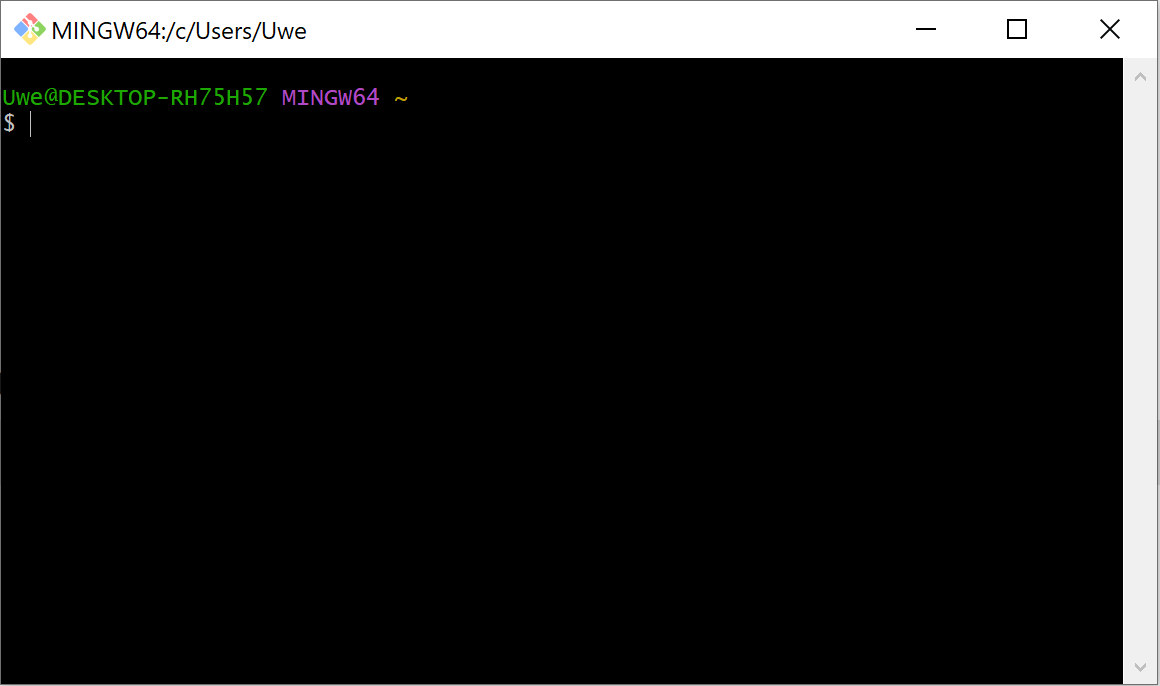
\includegraphics[width=\textwidth]{mingw-01}
\end{frame}
 
\begin{frame}
\frametitle{MinGW}

\begin{itemize}
\item MinGW = Minimal GNU\footnote{\enquote{GNU is not Unix} = Open-Source stuff} for Windows
\item A shell that ports many Unix/Linux tools to Windows
\item This is not Git, Git is just a commandline tool that can be used within MinGW
\item It contains a few Linux tools as well
\item To move in this MinGW environment you need to use Linux commands
\end{itemize}
\end{frame}

\begin{frame}
\frametitle{Basic MinGW commands}

\begin{description}
\item [pwd] In which directory are we?
\item [ls] List all files and folders
\item [cd] go to some specific directory
\item [mkdir] create a new directory
\end{description}

Remarks:

\begin{itemize}
\item There are no drive letters in MinGW
\item \texttt{/} is the root directory
\item Windows drive letters are (invisible) directories below this root directory
\item so \texttt{cd /c} takes you to the C:\textbackslash directory
\end{itemize}

\end{frame}

\section{Git}

\begin{frame}[containsverbatim]
\frametitle{Create new Repositories}

Create a directory, change to that directory and init the repository. The directory may already contains some files

\begin{lstlisting}
cd /e # go to the e: drive

mkdir myfirstgitrepo # create empty directory

cd myfirstgitrepo #  go to the directory

git init . # create repo (with a 'master' branch)
\end{lstlisting}

\end{frame}

\begin{frame}[containsverbatim]
\frametitle{git status}

Use \texttt{git status} whenever you want to know something about the current state of the repository

\begin{lstlisting}
Uwe@DESKTOP MINGW64 /e/myfirstgitrepo (master)
$ git status
On branch master

No commits yet

nothing to commit (create/copy files and use
"git add" to track)
\end{lstlisting}

\end{frame}

\begin{frame}[containsverbatim]
\frametitle{Adding files to the Repository 1} % create/copy files and use "git add" to track

\begin{lstlisting}
$ touch README.MD # creates an empty file

$ git status
On branch master

No commits yet

Untracked files:
(use "git add <file>..." to include in what will 
be committed)
        README.MD

nothing added to commit but untracked files 
present (use "git add" to track)
\end{lstlisting}

\end{frame}


\begin{frame}[containsverbatim]
\frametitle{Adding files to the Repository 2} 

\begin{lstlisting}
$ git add README.MD # add file to staging area

$ git add -A # add all files to staging area
# not added to repository

$ git reset # remove everything from the
# staging area

$ git commit -m "My message" # Don't forget!!!
\end{lstlisting}

\end{frame}


\begin{frame}[containsverbatim]
\frametitle{Adding files to the Repository 3} 

\begin{lstlisting}
$ git commit -m "Initial commit"
Author identity unknown

*** Please tell me who you are.

Run

  git config --global user.email "you@examp.de"
  git config --global user.name "Your Name"

to set your account's default identity.
Omit --global to set the identity only in this 
repository.

fatal: unable to auto-detect email address (got 
'Uwe@DESKTOP-RH75H57.(none)')
\end{lstlisting}

\end{frame}


\begin{frame}[containsverbatim]
\frametitle{Adding files to the Repository 4} 

\begin{lstlisting}[basicstyle=\ttfamily\scriptsize]
Uwe@DESKTOP MINGW64 /e/myfirstgitrepo (master)
$ git config --global user.email "ziegenhagen@gmail.com"

Uwe@DESKTOP MINGW64 /e/myfirstgitrepo (master)
$ git config --global user.name "Uwe Ziegenhagen"

Uwe@DESKTOP MINGW64 /e/myfirstgitrepo (master)
$ git commit -m "Initial commit"
[master (root-commit) acb9d75] Initial commit
 1 file changed, 0 insertions(+), 0 deletions(-)
 create mode 100644 README.MD

Uwe@DESKTOP MINGW64 /e/myfirstgitrepo (master)
$ git status
On branch master
nothing to commit, working tree clean
\end{lstlisting}

Now we have a file under version control! 

\end{frame}


 
\end{document}